\section{Deep Q-Learning}
\subsection{Motivation}
The greatest constraint of the Q-learning implementation is the spatial complexity of the \emph{Q-table}. 
The maximum size of the \emph{Q-table} is the product of possible states and possible actions, given by:

\[ |Q_{full}| = min(11, m + 3)^{n^2} \times n^2 \]

Where $n$ is the board size and $m$ is the number of mines.
The value 11 indicates the number of possible values in any cell, ranging from -2 to 8, as explained before.
Even by reducing the problem to a $4 \times 4$ board with 4 mines, a filled \emph{Q-table} would have $7^{16} \times 16 \approx 5.3 \times 10^{14}$ values.
Although a successful agent will not need a full \emph{Q-table}, the Q-learning implementation requires both more training time and more storage to produce desirable results.
This limitation served as a motivation to move towards addressing the problem with a deep Q-learning model.

\subsection{Method} % implementation?

The deep Q-learning algorithm replaces the previous Q-table with a neural network to predict Q-values based on the current state to choose the best action. A simple 5-layered neural network is used (shown in Appendix C). The Bellman equation is now simpler, excluding the hyperparameter learning rate (since the back-propagation in the neural network already has it optimized by an optimizer) \cite{tds}:

\setlength\parindent{15pt}
\[
 Q'(s,a)
  = \cancel{Q(s,a)}
  + \cancel{\alpha}
  [ R(s,a)
  + \gamma
  maxQ(s',a')
  - \cancel{Q(s, a)}] 
\]
\[Q'(s,a) 
    = R(s,a) + \gamma maxQ(s',a')
\]
\setlength\parindent{0pt}

The rest of the tuned hyperparameter values are used. As the agent gets trained, it stores its experience in a sequential memory with a certain limit, and this experience is used to further train the agent. The current neural network predicts the Q-values for the old state, and the new state by taking a certain action. Then, a new set of target Q-values is calculated using the bellman equation, and the neural network can be further trained with the old state as the input, and the target Q-values as the output. The rest of the Q-learning algorithm stays the same.

\subsection{Results}

\begin{figure}[H]
\centering
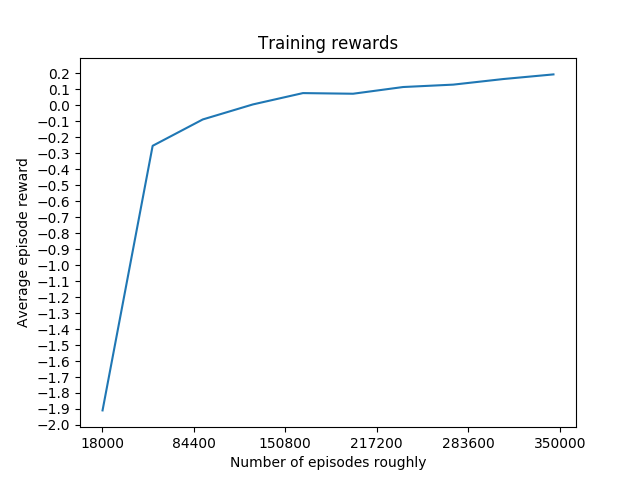
\includegraphics[width=0.65\textwidth]{dql-results.png}
\caption{Deep Q-Learning reward vs. training episodes}
\end{figure}
As seen in the plot, the reward increases at a higher rate at the beginning of training, then increases steadily. After being trained for roughly 350,000 episodes (1,900,000 steps), the agent achieves a reward of 0.194. If trained for more time, the reward will still likely increase, but due to the long training hours, we stopped at 350,000 episodes to see how it performs against the normal Q-agent. After testing for 86,000 episodes, it achieves an average reward of 0.3854, a winning percentage of 16.87\%, and a board completion rate of 42.7\%.
\\\\
Compared with the normal Q-agent, the average reward is generally lower possibly because the deep agent has not yet completely learned to not step on the same cell repeatedly judging from its visualization, receiving negative rewards. Moreover, the normal Q-agent manages to achieve a higher board completion rate. However, one should note that the deep agent is trained for about 23 times fewer episodes within roughly the same amount of time of 8 hours, and still achieves a higher winning percentage. 
